%!TEX root = ../thesis.tex

\fxnote[inline, nomargin]{Note that the same/similar things hold for the left boundary walk. However we do not need this. So do I mention it?}

\section{The right neighbor path of a path}
  \label{s:rightNeighbour}
  Before we can define anything in this section we first need to carefully define what the right of a path is, hence we introduce the notion of rotations at a vertex. During the proofs in this section we will also need various types of chords and thus we also introduce more information on chords

  \mypar{Rotations}
    We assume a fixed embedding for $G$. In this embedding the \emph{rotation} at a vertex $v$ is the clockwise order of the edges incident to $v$. We will identify these edges with their other endpoints.
    Two vertices $x, y$ are said to be \emph{consecutive} in the rotation at $v$ when the edges $vx$ and $vy$ are consecutive in the rotation.
    We sometimes want to denote number of subsequent vertices or \emph{interval} in the rotation. We let $[x,y]$ denote all the vertices in the rotation of $v$ from $x$ to $y$ and we let the \emph{exclusive interval} $(x,y)$ denote the same vertices without $x$ or $y$.
    Given a path $P$ and a interior vertex $p_i$. A neighbor $v \nin \P$ of $p_i$ lies on the \emph{left} of $P$ if it lies in the interval from $p_{i-1}$ to $p_{i+1}$ in the clockwise rotation at $p_{i}$. Otherwise $v$ lies in the interval from $p_{i+1}$ to $p_{i-1}$ in the rotation clockwise at $p_i$. In this case $v$ lies on the \emph{right} of $P$.
    We will use the same notion of left and right for edges. That is, an edge $e\nin P$ adjacent to $p_i$ lies to left or right if its other end point lies to the left or right, respectively. In Figure \ref{fig:right:rot} $v$ lies on the left of $P$ and $u$ lies on the right of $P$.

    \begin{figure}[h]
      \centering
      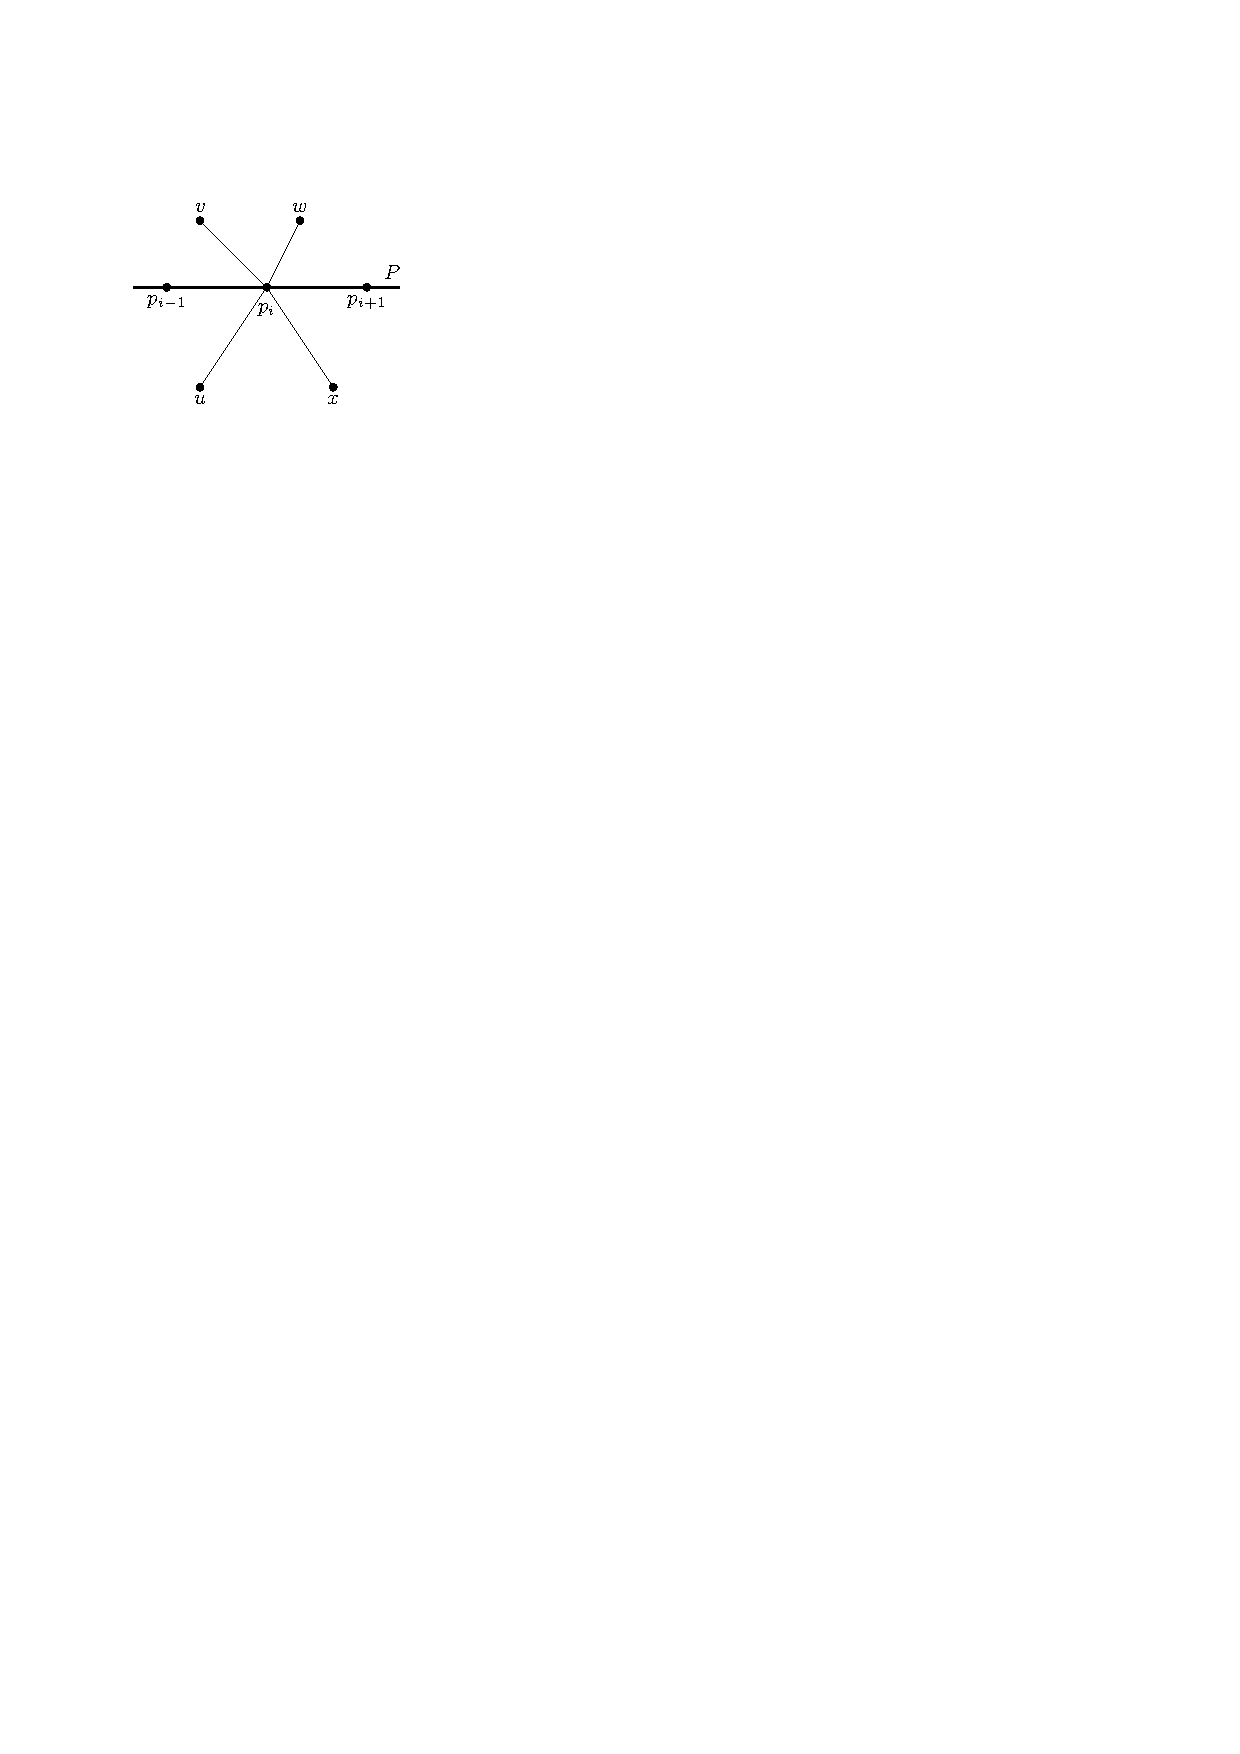
\includegraphics[scale=1]{unifiedAlgo/img/rightNeighbourwalk/rotation}
      \caption{}
      \label{fig:right:rot}
    \end{figure}

  \mypar{Chords}
    A \emph{chord} of a path is an edge that connects two vertices in this path, but is not part of the path. A path without chords is \emph{chordfree}.
    A \emph{k-chord} is a path $\Q$ of length $k$ that connects two non-subsequent vertices $p_i, p_j$ of $\P$ such that $\P \cap \Q = \braces{p_i, p_j}$.
    Since a cycle is a special type of path the same definitions also apply to them.
    Note that $\P|_{v_i, v_j} \oplus \rev{\Q}$ is a cycle. The ($k$-)chord $\Q$ is \emph{separating} if this cycle is separating.

  \mypar{Right neighbor paths}
    In the sweepcycle step of the algorithm (Section \ref{s:sweep}) we will use the right neighbor path of a path. We show that given a path $P = p_1 \ldots p_k$ whose interior vertices are not incident to the outer face and without chords or separating 2-chords on the right of the path. The the right neighbors of $P$ are again a path (Lemma \ref{lm:uni:neighborWalk}).

    \begin{lemma}
      \label{lm:right:pHasRightNeihgbours}
      Every interior vertex of $P$ has at least one neighboring vertex on the right.
    \end{lemma}

    \begin{proof}
      Suppose that a interior vertex $p_i$ has no neighbor on the right of the path. Then $ \ldots p_{i-1} p_i p_{i+1} \ldots $ is a partial face border. Since $p_i$ is not incident to the outer face $p_i$ must be incident to a face of degree $3$. Thus $p_{i-1} p_i p_{i+1}$ is a face. However, this would imply a chord on the right of $P$ as can be seen in Figure \ref{fig:right:pHasRightNeighbor}. Hence by contradiction $p_i$ must have a neighbor on the right.
    \end{proof}

    \begin{figure}[h]
      \centering
      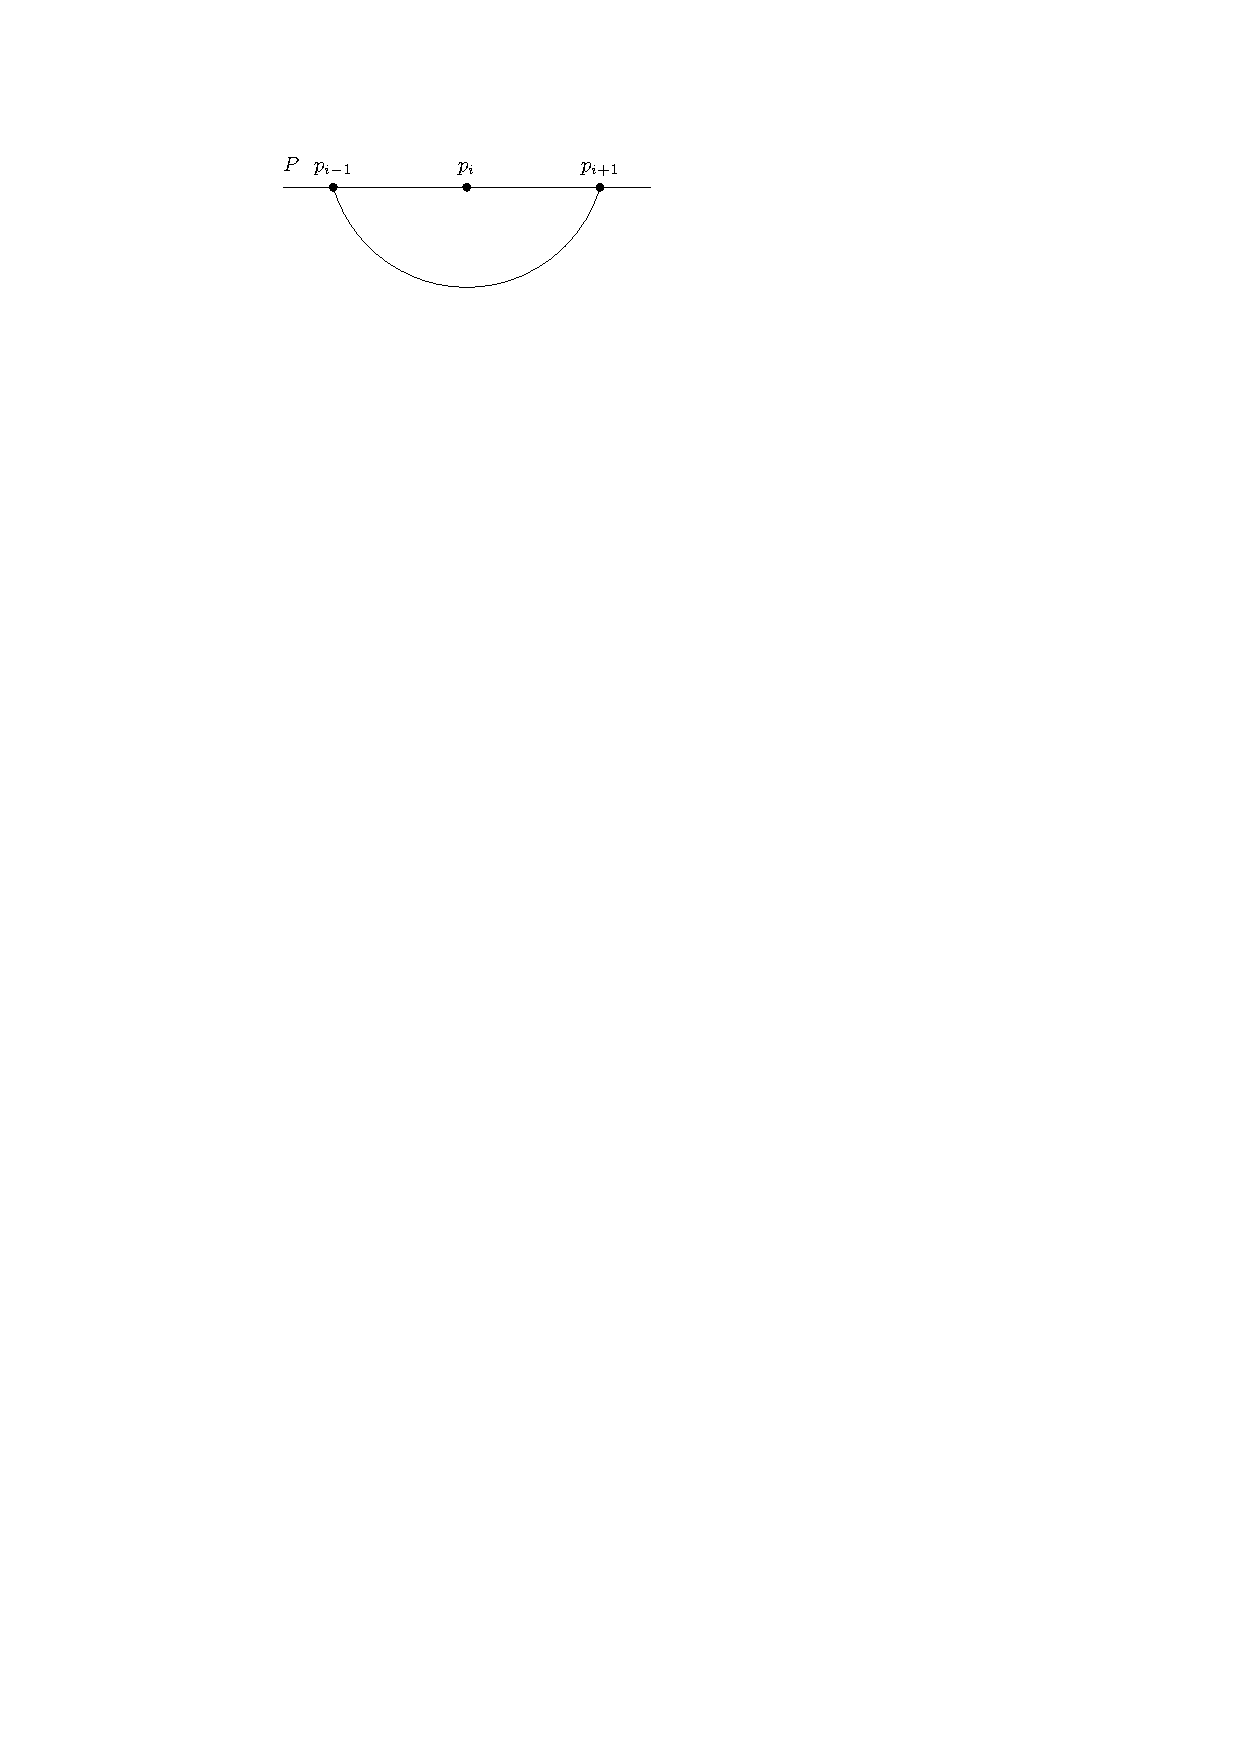
\includegraphics[scale=1]{unifiedAlgo/img/rightNeighbourwalk/pHasRightNeighbor.pdf}
      \caption{}
      \label{fig:right:pHasRightNeighbor}
    \end{figure}

    These right neighbors of $P$ will form the the \emph{right neighbor path} $Q$ of $P$.
    Let us first define a larger list of vertices $Q'$. $Q'$ will consist of $p_1$ and those vertices adjacent to $p_{2}$ that are in the exclusive interval $(p_1, p_3)$ of the clockwise rotation at $p_2$. Followed by the vertices in the interval $(p_2, p_4)$ of the rotation at $p_{3}$. We continue this up to the vertices in the interval $(p_{k-2}, p_k)$ of the rotation at $p_{k-1}$ and finally $p_k$.
    We obtain $Q$ from $Q'$ by removing all subsequent duplicates from $Q$.
    In Figure \ref{fig:right:neighborPath} an example of a right neighbor path is given.

    \fxnote{Q: figure  \ref{fig:right:neighborPath}  with or without half edges on the borders?}
    \begin{figure}[h]
      \centering
      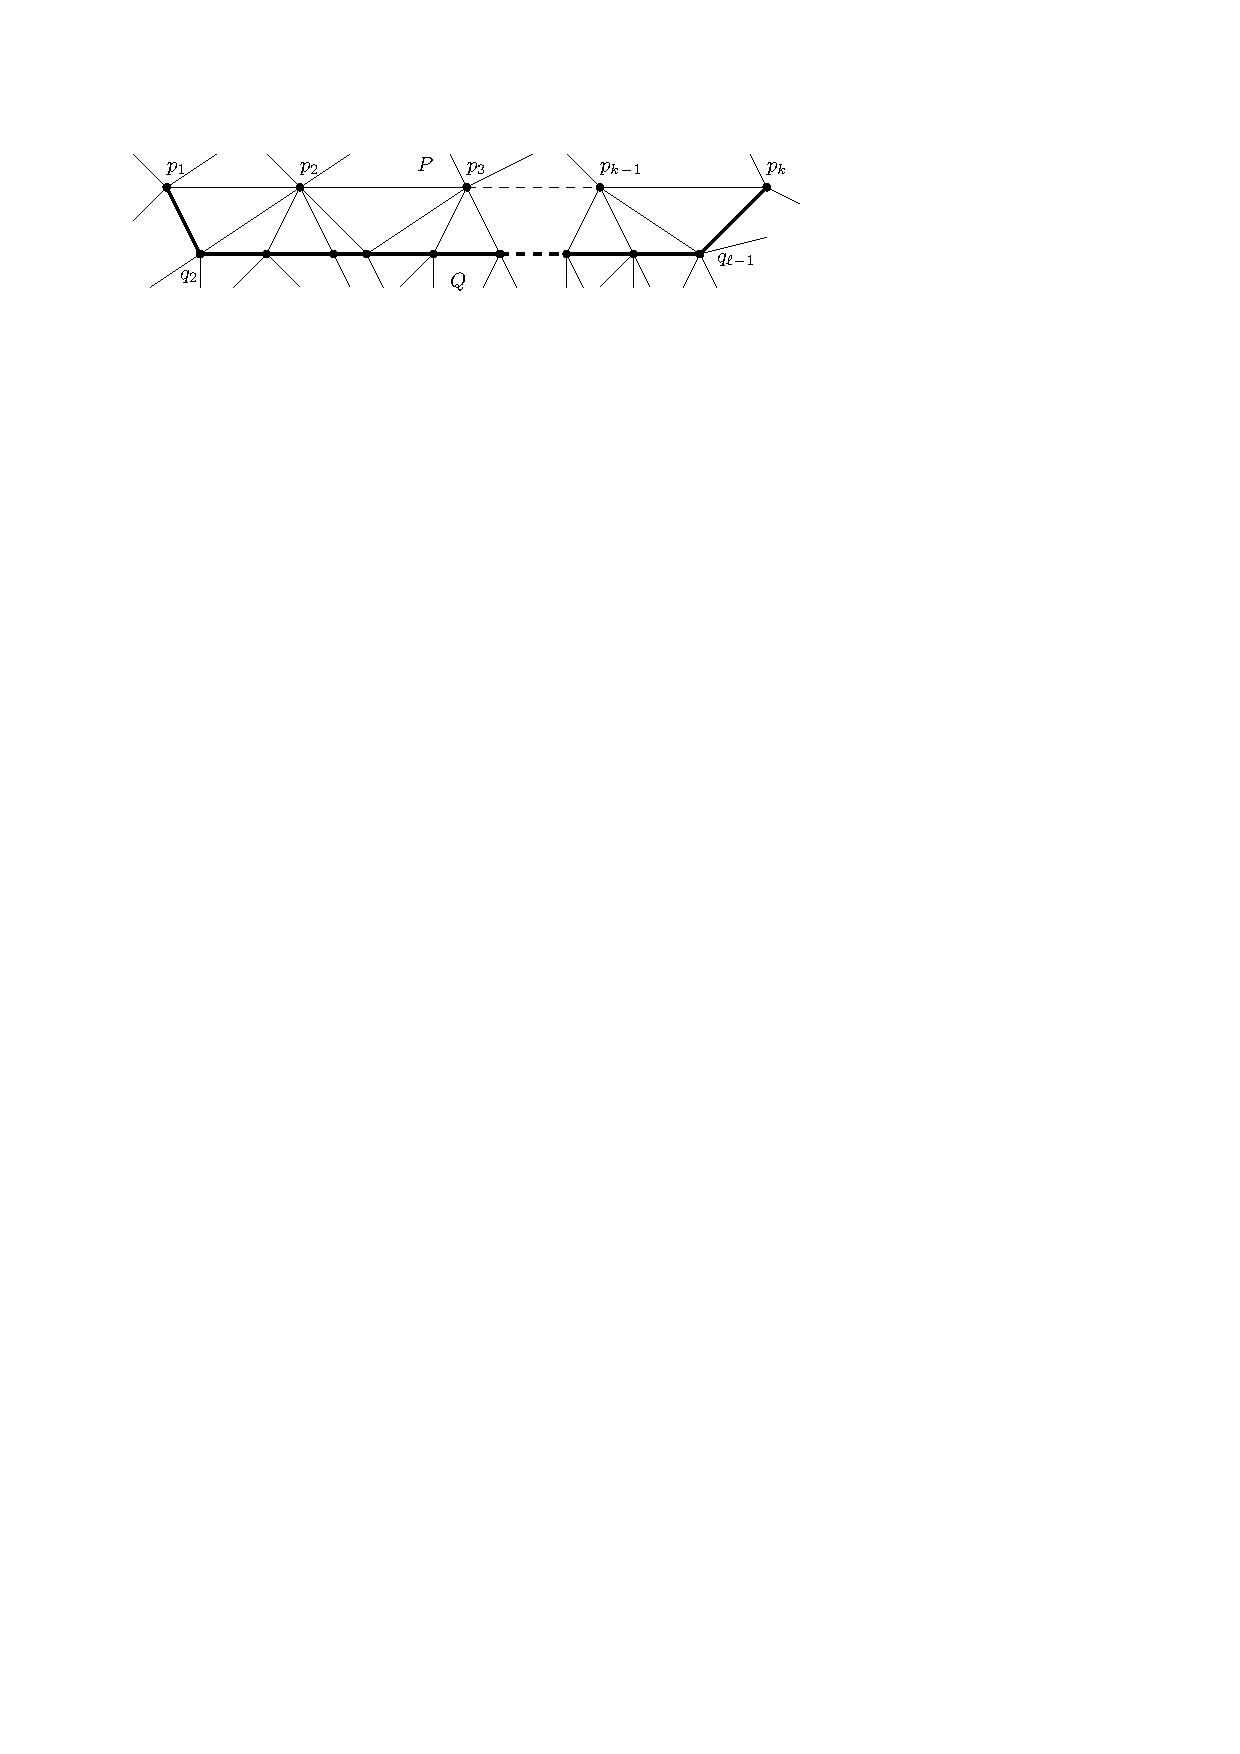
\includegraphics[scale=1]{unifiedAlgo/img/rightNeighbourwalk/neighborPath.pdf}
      \caption{}
      \label{fig:right:neighborPath}
    \end{figure}


  \fxnote{Walk is not yet defined}
  \begin{lemma}
    \label{lm:uni:neighborWalk}
    The right neighbor path $Q$ is a walk.
  \end{lemma}
  \begin{proof}
    Let $q_i$ and $q_{i+1}$ be two subsequent vertices of $Q'$. We will show they are either connected or the same vertex. We first consider the case where $1 < i < k-1$.
    Now there are two sub-cases. Either $(a)$ $q_i$ and $ q_{i+1}$ are vertices adjacent to the same vertex $p_j$ an thus subsequent in the rotation at $p_j$ or $(b)$ $q_i$ was the last vertex adjacent to $p_j$ and thus $q_{i+1}$ is the first vertex adjacent to $p_{j+1}$ since by Lemma \ref{lm:right:pHasRightNeihgbours} every interior vertex of $P$ has right neighbors.

    \begin{figure}[h]
      \centering
      \begin{subfigure}[b]{0.5\linewidth}
          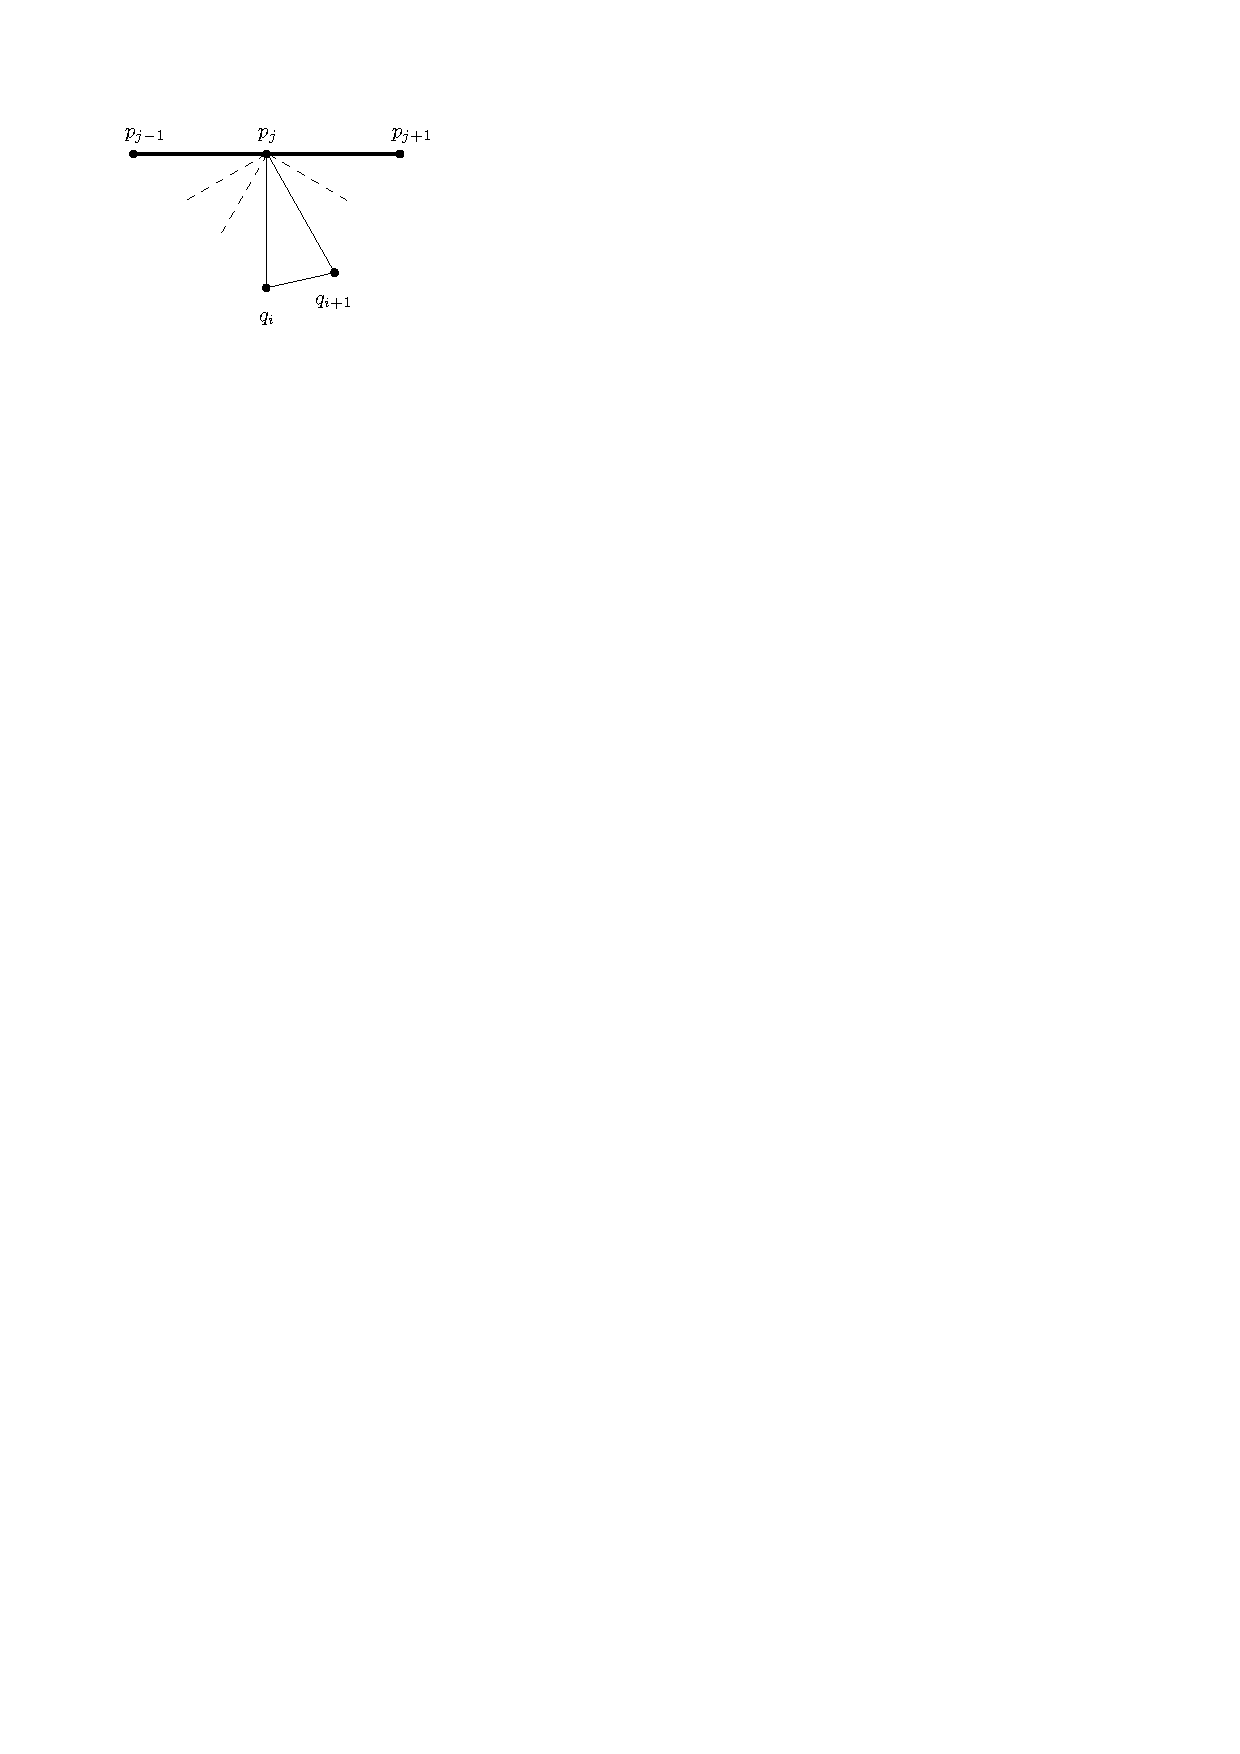
\includegraphics[width=\linewidth]{unifiedAlgo/img/walkProofA}
          \caption{}
      \end{subfigure}%
      \begin{subfigure}[b]{0.5\linewidth}
          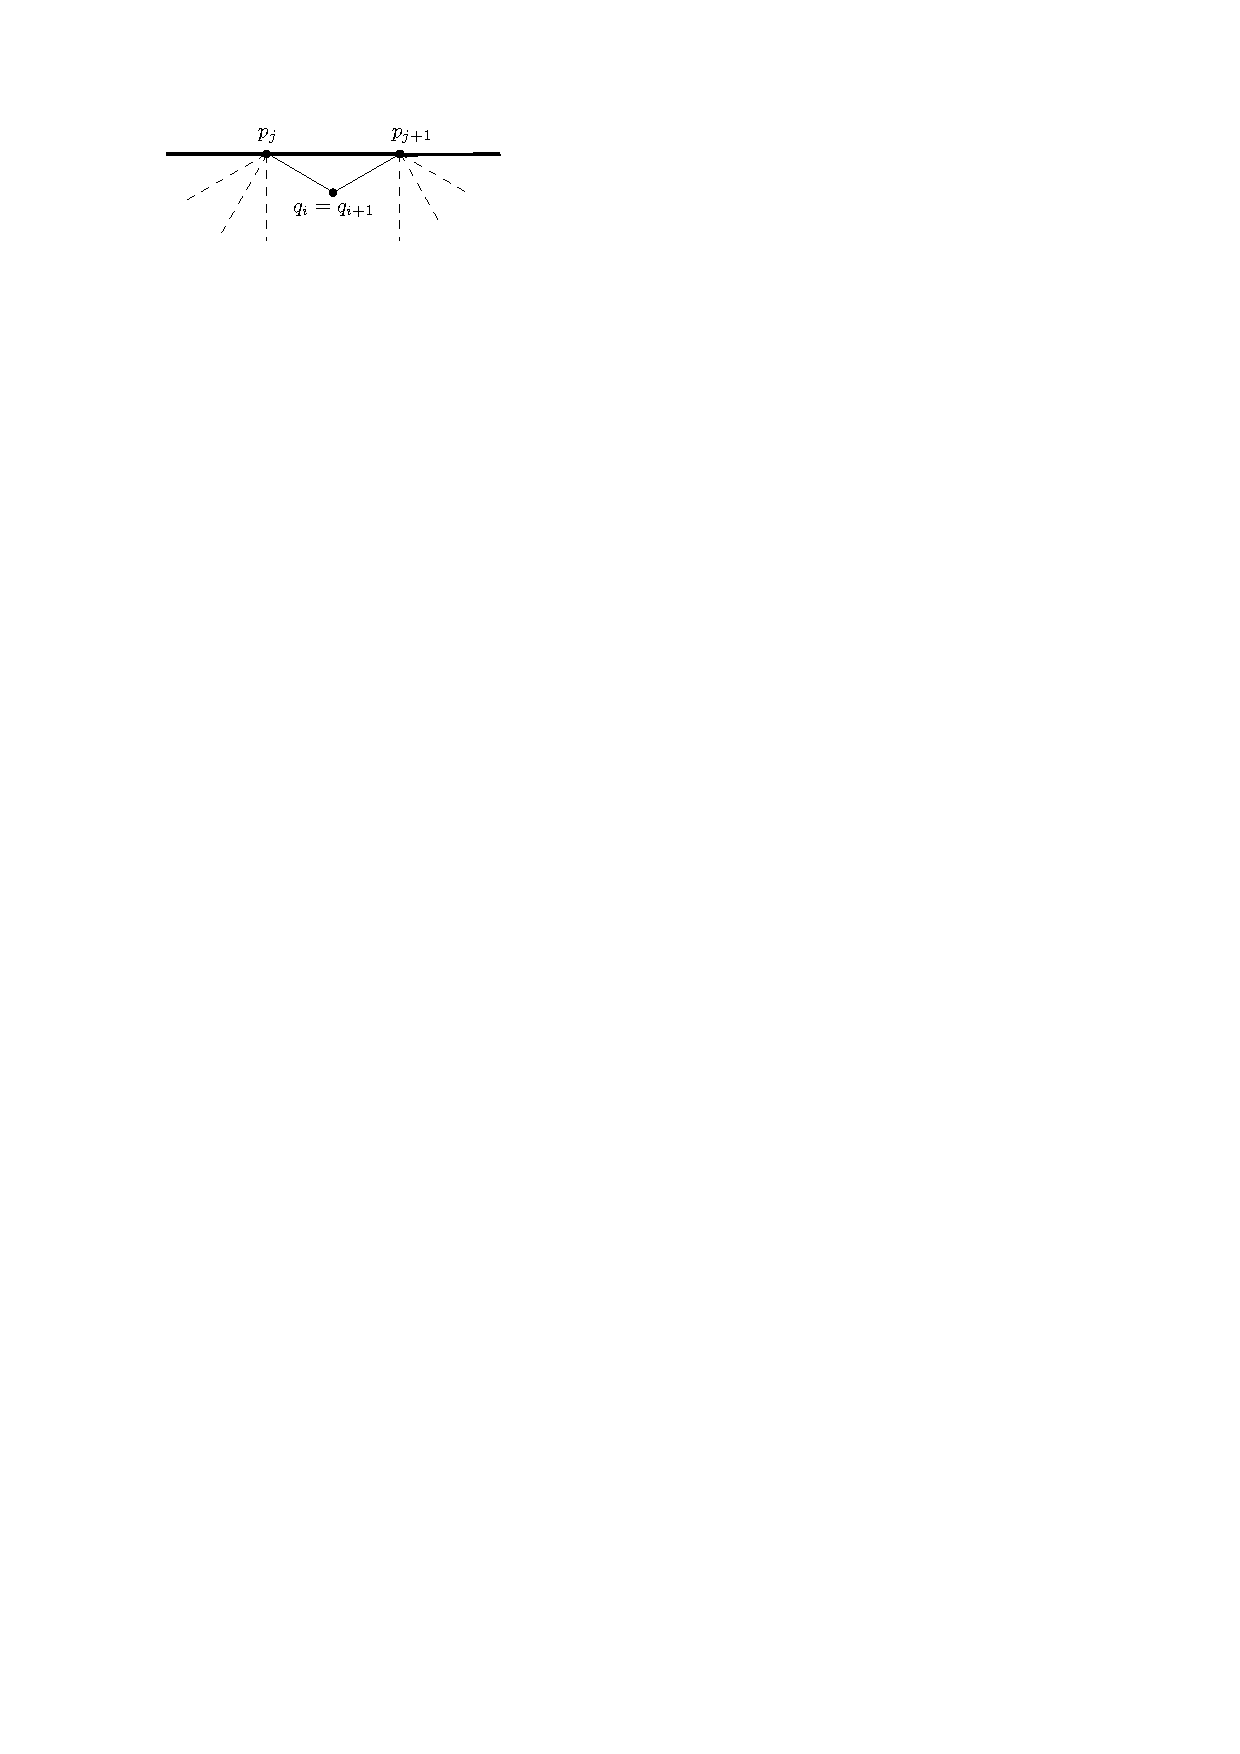
\includegraphics[width=\linewidth]{unifiedAlgo/img/walkProofB}
          \vspace{1cm}
          \caption{}
      \end{subfigure}
      \caption{The two main cases of the proof showing that $W$ is a walk}
      \label{fig:uni:walkproof}
    \end{figure}

    In case $(a)$ we note that since $q_i$ and $q_{i+1}$ are subsequent in the rotation at $p_j$ $q_i q_{i+1}$ is an edge since $p_j$ is not incident to the outer face and every interior face of $G$ is a triangle.

    In case $(b)$ we note that $p_i q_i$ and $p_i p_{i+1}$ are edges subsequent in clockwise order, hence $q_{i} p_{i+1}$ is also an edge. Hence $q_i$ is the first vertex adjacent to $p_{i+1}$ subsequent to $v_i$ in the clockwise rotation. Thus $q_{i} = q_{i+1}$. They are duplicates.

    Now for the cases $i=1$ and $i=k-1$. $q_1$ and $q_2$ are vertices adjacent to $p_{2}$ subsequent in the clockwise rotation of ${p_2}$, and hence connected since every interior face is a triangle. In the same way $q_{k-1}$ and $q_k$ are subsequent vertices in the rotation at $q_{k-1}$ and hence connected.
    \fxnote{Add figure of the cases $i=1$ and $i=k-1$}

    Since all pairs of subsequent vertices in $Q'$ are connected or duplicates $Q$ is a walk.
  \end{proof}

  \begin{lemma}
    \label{lm:uni:neighborPath}
    The right neighbor path $Q$ is a path
  \end{lemma}
  \begin{proof}
    We already know $Q$ is a path by \ref{lm:uni:neighborWalk}. Hence we only have to show that $Q$ contains no duplicate vertices.

    Suppose that $Q$ has a duplicate vertex $q_i=q_j$ with $i<j$. Then this vertex must have been a neighbor to two different vertices in $P$. We denote these vertices $p_i$, $p_j$ with $i<j$. We are now in the situation of Figure \ref{fig:right:path}.

    By the order in which we added vertices to $Q'$, which is preserved by the removal of when we go to $Q$, we know that any vertices in-between $q_i$ and $q_j$ must be one of the following: $1)$ Adjacent to $p_i$ and in the interval $(q_i, p_{i+1})$ in $p_i$'s rotation. $2)$ Adjacent to one of $p_{i+1},  p_{i+2},\ldots, p_{j-1}$ and to the right of $P$. $3)$ Adjacent to $p_j$ and in the interval $(p_{j-1}, q_j)$ in $p_j$'s rotation.

    All of the three cases describe a vertex that must lie in the interior of the cycle $q_i p_i p_{i+1} \ldots p_j$. However, since $P$ has no separating $2$-chords on the right this cycle must be empty. Therefore there are no vertices in-between $q_i$ and $q_j$ but since $Q$ is a walk and $G$ is simple $Q$ can't contain any subsequent duplicates. Hence $Q$ contains no duplicates and $Q$ is thus a path.
  \end{proof}

  \begin{figure}[h]
    \centering
    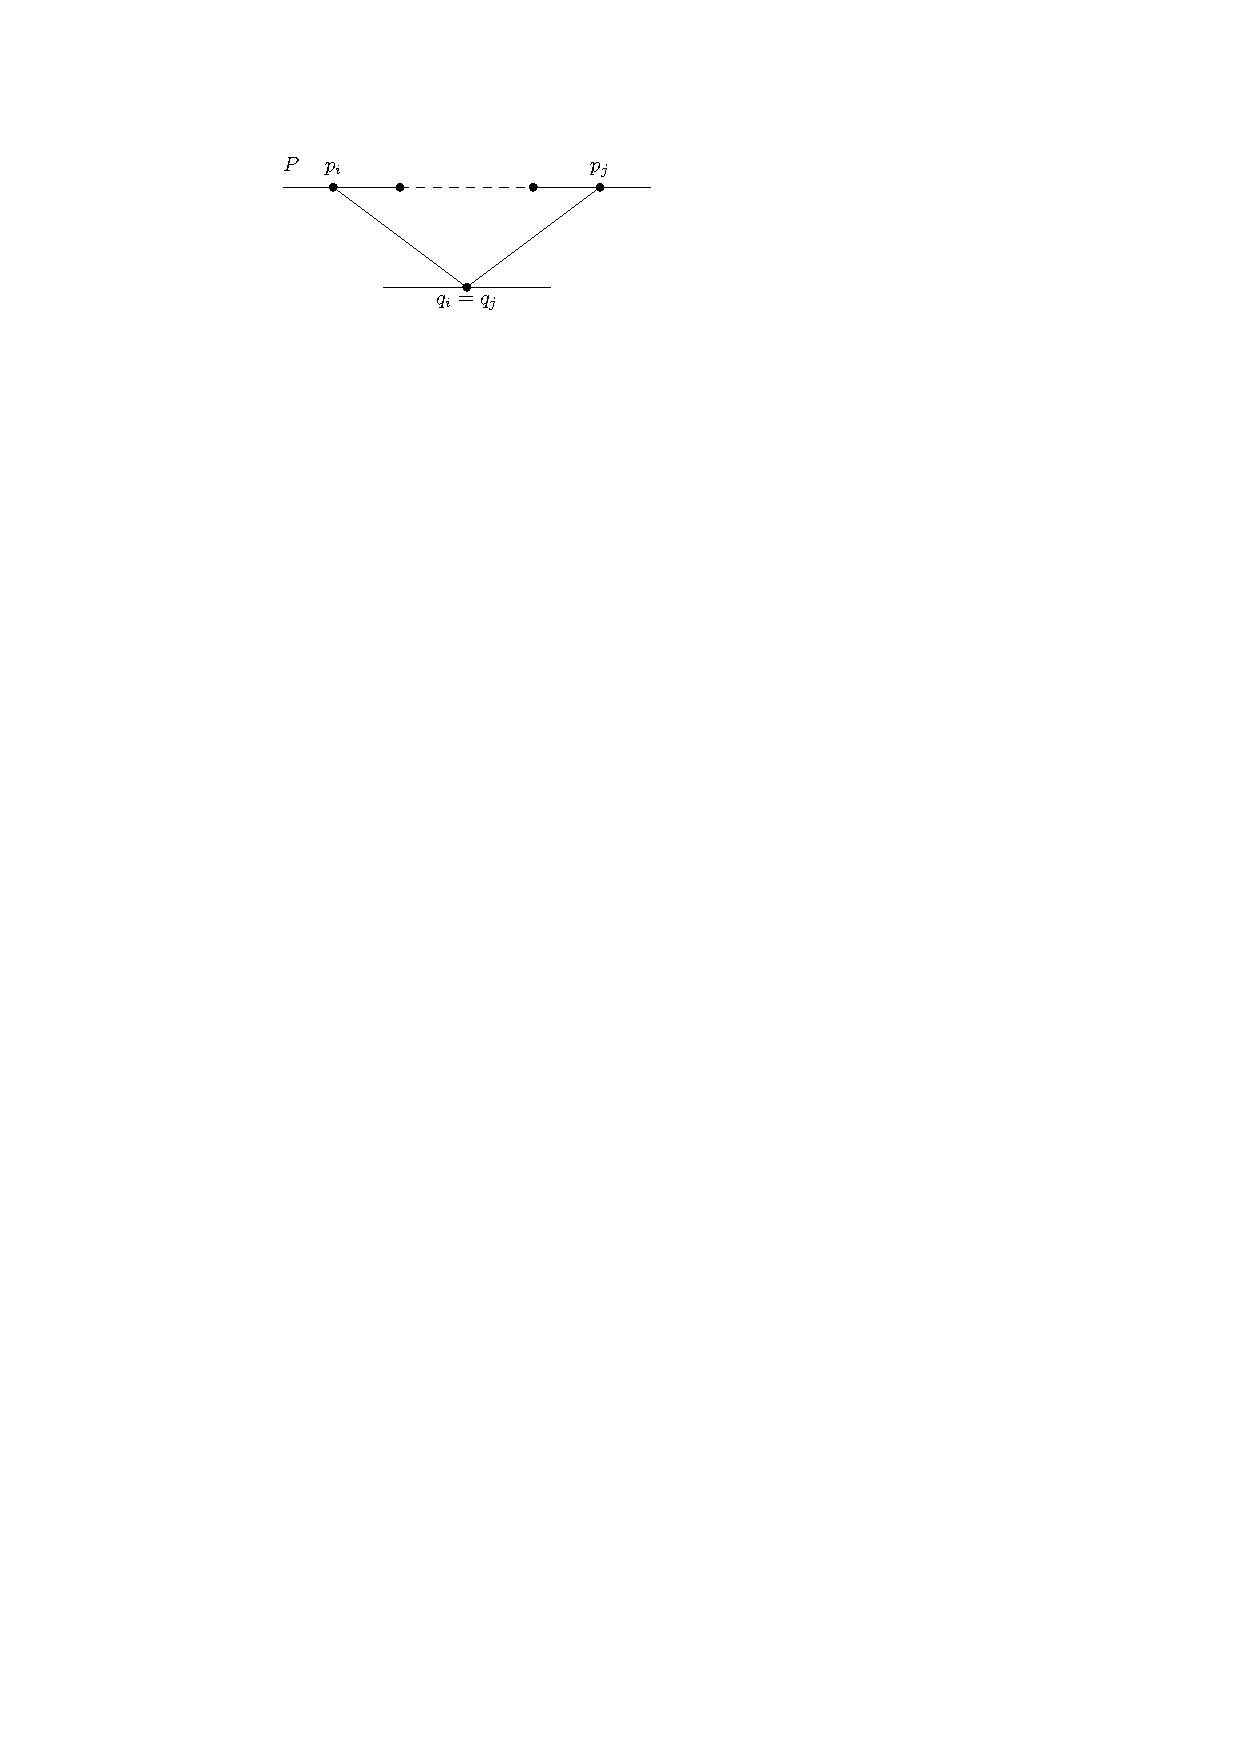
\includegraphics[scale=1]{unifiedAlgo/img/rightNeighbourwalk/neighborPathisPath.pdf}
    \caption{}
    \label{fig:right:path}
  \end{figure}

  \fxinnote{Concat notation}
  \begin{lemma}
    \label{lm:uni:neighbourwalkNoInteriorVertex}
    The cycle $P \oplus \rev{Q}$ has no interior vertices.
  \end{lemma}
  \begin{proof}
    The interior of $W \oplus \rev{P}$ consists of only triangles with all vertices in $W \oplus \rev{P}$. We can see this from the construction of the neighbor path. Both cases in Figure \ref{fig:uni:walkproof} add a triangle to the interior with all vertices in $W \oplus \rev{P}$.

    Suppose there is a interior vertex. Then the triangle containing this vertex is a separating triangle.
    \fxnote{This is hardly formal}
  \end{proof}


  \begin{lemma}
    \label{lm:uni:neighbourwalkChordFree}
    The left of a right neighbor path is chordfree.
  \end{lemma}
  \begin{proof}
    Suppose that the right neighbor path $Q = q_1 \ldots q_k$  has a chord on the left, say between $q_i$ and $q_j$ with $i< j -1 $. There is a vertex $p_\ell \in P$ on the path such that $q_{i+1}$ is a neighbor of $p_\ell$ to the left of $p_\ell$. Consider now the cycle $P q_k \ldots q_{j+1} q_j q_i q_{i-1} \ldots q_1$
    (Thick in Figure \ref{fig:uni:neihbourwalkChordFree})this cycle has $q_{i+1}$ in its exterior. But then $p_\ell w_{i+1}$ is a crossing edge. Which is forbidden.
    %\fxnote{Alternate proof based on   ($\W$ being oriented from $\pW$ to $\pE$), since if it would lie on the left of $\W$ the vertices $w_{i+1},\ldots, w_{j-1}$ would not have been chosen in the construction of the prefence.}

    \begin{figure}[h]
      \centering
      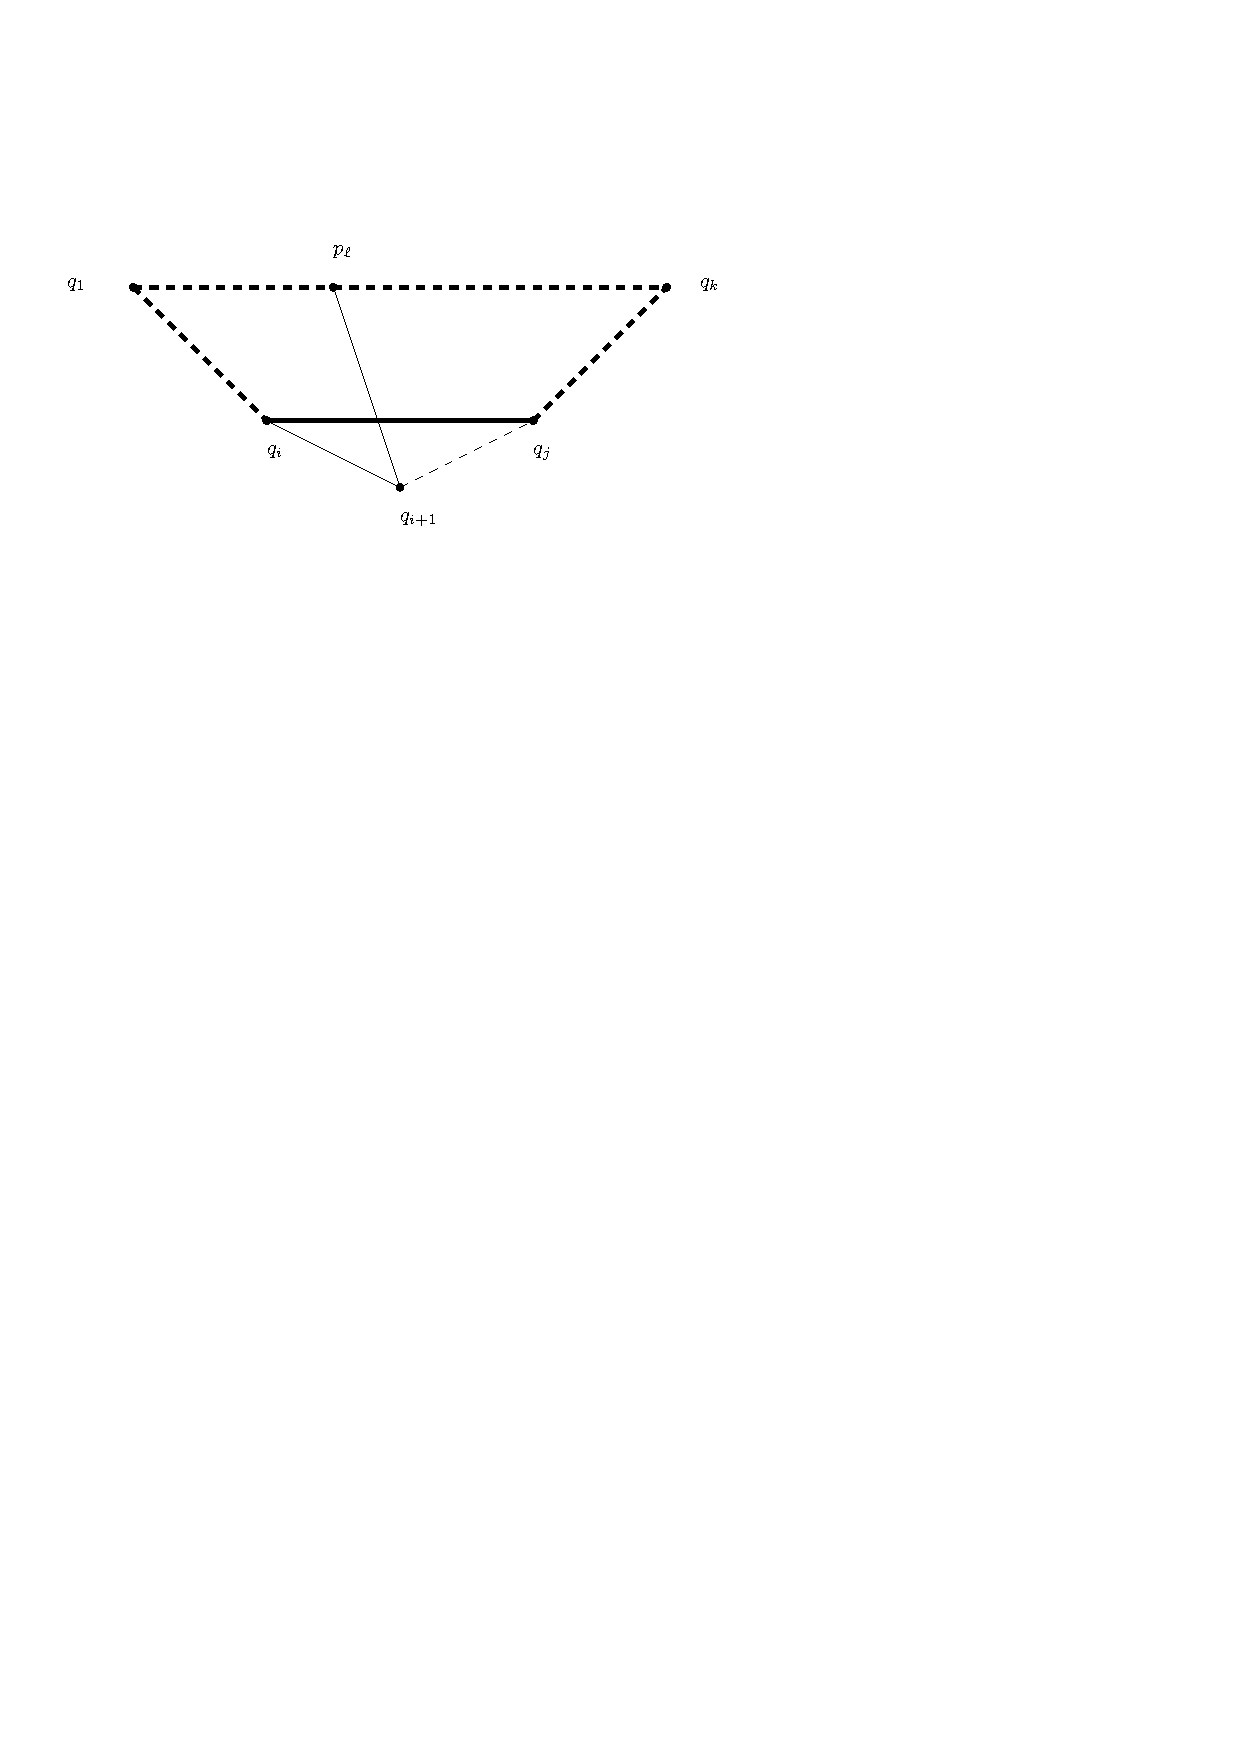
\includegraphics[scale=1]{unifiedAlgo/img/neighbourWalkChords}
      \caption{The construction in the proof of Lemma \ref{lm:uni:neighbourwalkChordFree}}
      \label{fig:uni:neihbourwalkChordFree}
    \end{figure}
  \end{proof}
